% Build:  cd presentation && tectonic main.tex
% (needs the `abcfold-npf-presentation` conda env — see ../envs/presentation.yaml)
\documentclass[aspectratio=169]{beamer}

\usetheme{default}
\usepackage[utf8]{inputenc}
\usepackage{tikz}
\usetikzlibrary{arrows.meta, positioning, fit}
\usepackage{booktabs}
\usepackage{graphicx}
\graphicspath{{figures/}{figures/background/}{figures/logos/}{figures/license/}}

% --- Dark palette (Solarized Dark) --------------------------------------
\definecolor{bgdark}{HTML}{002B36}
\definecolor{fgtext}{HTML}{93A1A1}
\definecolor{accent}{HTML}{2AA198}   % structure/links/bullets
\definecolor{muted}{HTML}{586E75}   % footline / secondary text
\definecolor{lobeN}{HTML}{268BD2}    % MFS icon: N-domain lobe
\definecolor{lobeC}{HTML}{CB4B16}    % MFS icon: C-domain lobe
\definecolor{substrate}{HTML}{D33682} % MFS icon: bound-substrate dot

% MFS conformation icon: two elongated lobes (N, C) hinged at a shared
% pivot (0,0) -- the domain interface/gate. Each lobe rotates AROUND that
% pivot, N by +#3 and C by -#3, so a nonzero #3 splays them apart on one
% side (a V-shaped opening) while the other side stays pinched shut --
% this is the rocker-switch motion itself, not a rigid icon tilt.
% #1,#2 = position; #3 = signed splay angle in degrees
%   (0 = occluded/upright, +ve = opens upward/outward, -ve = opens downward/inward)
% #4 = extra draw code, e.g. a substrate dot, or empty
\newcommand{\mfsicon}[4]{%
  \begin{scope}[shift={(#1,#2)}]
    \begin{scope}[rotate around={#3:(0,0)}]
      \filldraw[fill=lobeN, draw=fgtext, line width=0.4pt] (-0.26,0) ellipse (0.27 and 0.58);
      \node[white, font=\bfseries\tiny] at (-0.26,0) {N};
    \end{scope}
    \begin{scope}[rotate around={-#3:(0,0)}]
      \filldraw[fill=lobeC, draw=fgtext, line width=0.4pt] (0.26,0) ellipse (0.27 and 0.58);
      \node[white, font=\bfseries\tiny] at (0.26,0) {C};
    \end{scope}
    #4
  \end{scope}%
}

\setbeamertemplate{navigation symbols}{}
\setbeamercolor{background canvas}{bg=bgdark}
\setbeamercolor{normal text}{fg=fgtext, bg=bgdark}
\setbeamercolor{structure}{fg=accent}
\setbeamercolor{title}{fg=fgtext}
\setbeamercolor{subtitle}{fg=muted}
\setbeamercolor{author}{fg=muted}
\setbeamercolor{institute}{fg=muted}
\setbeamercolor{date}{fg=muted}
\setbeamercolor{frametitle}{fg=fgtext, bg=bgdark}
\setbeamercolor{itemize item}{fg=accent}
\setbeamercolor{itemize subitem}{fg=accent}
\setbeamercolor{enumerate item}{fg=accent}
\setbeamertemplate{itemize item}[circle]
\setbeamertemplate{itemize subitem}[circle]
\setbeamercolor{section in toc}{fg=fgtext}
\setbeamercolor{page number in head/foot}{fg=muted}
\setbeamerfont{frametitle}{series=\bfseries}
\setbeamercolor{footlineright}{fg=muted, bg=bgdark}
\setbeamertemplate{footline}{%
  \leavevmode%
  \hbox{%
    \begin{beamercolorbox}[wd=\paperwidth, ht=2.6ex, dp=1.2ex, right, rightskip=0.3cm]{footlineright}
      \usebeamerfont{footline}\tiny CC BY 4.0~\raisebox{-0.15em}{
\includegraphics[height=1.4ex]{by-4.0-88x31.pdf}}\hspace{0.4em}\insertframenumber\,/\,\inserttotalframenumber
    \end{beamercolorbox}%
  }%
}
% NOTE: \setbeamertemplate{itemize/enumerate body begin} does NOT control
% \itemsep in this beamer/theme combo (verified: even 40em had zero visual
% effect and zero overflow). Patching \@listi/\@listii directly -- the real
% LaTeX list-level macros -- is what actually works; \g@addto@macro appends
% our overrides without disturbing their existing leftmargin/etc.
% \itemsep spaces siblings apart (e.g. 1.1 <-> 1.2); \topsep spaces a nested
% list from its parent item (e.g. "1." <-> "1.1", and "1.2" <-> "2.").
% Also: beamer resets \@listi (depth 1 only, not \@listii) at
% \begin{document}, silently wiping a preamble-time patch -- wrapping ours
% in \AtBeginDocument makes it run after that reset instead of before it.
\makeatletter
\AtBeginDocument{%
  \g@addto@macro{\@listi}{\setlength{\itemsep}{1em}\setlength{\topsep}{1em}}
  \g@addto@macro{\@listii}{\setlength{\itemsep}{1em}\setlength{\topsep}{1em}}
}
\makeatother
\setbeamertemplate{sections/subsections in toc}[sections numbered]

\title{ABCfold NPF Conformation Pipeline}
\subtitle{Six structure-prediction backends, launched together, clustered by TM-helix alignment}
\author{Etienne Reboul}
\institute{Groupe Gibbérellines et adaptation à l'environnement\\
Institut de Biologie Moléculaire des Plantes (IBMP), Strasbourg}
\date{\today}

\begin{document}

\begin{frame}
  \begin{tikzpicture}[remember picture, overlay]
    \node[anchor=north] at ([yshift=-0.5cm]current page.north) {
      
\includegraphics[height=0.8cm]{cnrs-white.png}%
      \hspace{1.4cm}%
      {\setlength{\fboxsep}{4pt}\colorbox{white}{
\includegraphics[height=0.7cm]{ibmp-color.png}}}%
      \hspace{1.4cm}%
      
\includegraphics[height=0.8cm]{anr-white.png}
    };
  \end{tikzpicture}
  \titlepage
\end{frame}

\begin{frame}{Outline}
  \tableofcontents
\end{frame}

% ---------------------------------------------------------------------
\section{Background}
% ---------------------------------------------------------------------

\begin{frame}{Gibberellins}
  \begin{columns}[c]
    \begin{column}{0.55\textwidth}
      \begin{itemize}
        \item Key phytohormone in plants; isolated in 1931 from
          \textit{Gibberella fujikuroi} (fungus), later found in plants
          (1950)
        \item Promotes growth and development:
          \begin{itemize}
            \item Stem elongation
            \item Seed germination
            \item Flowering
          \end{itemize}
      \end{itemize}
    \end{column}
    \begin{column}{0.42\textwidth}
      \centering
      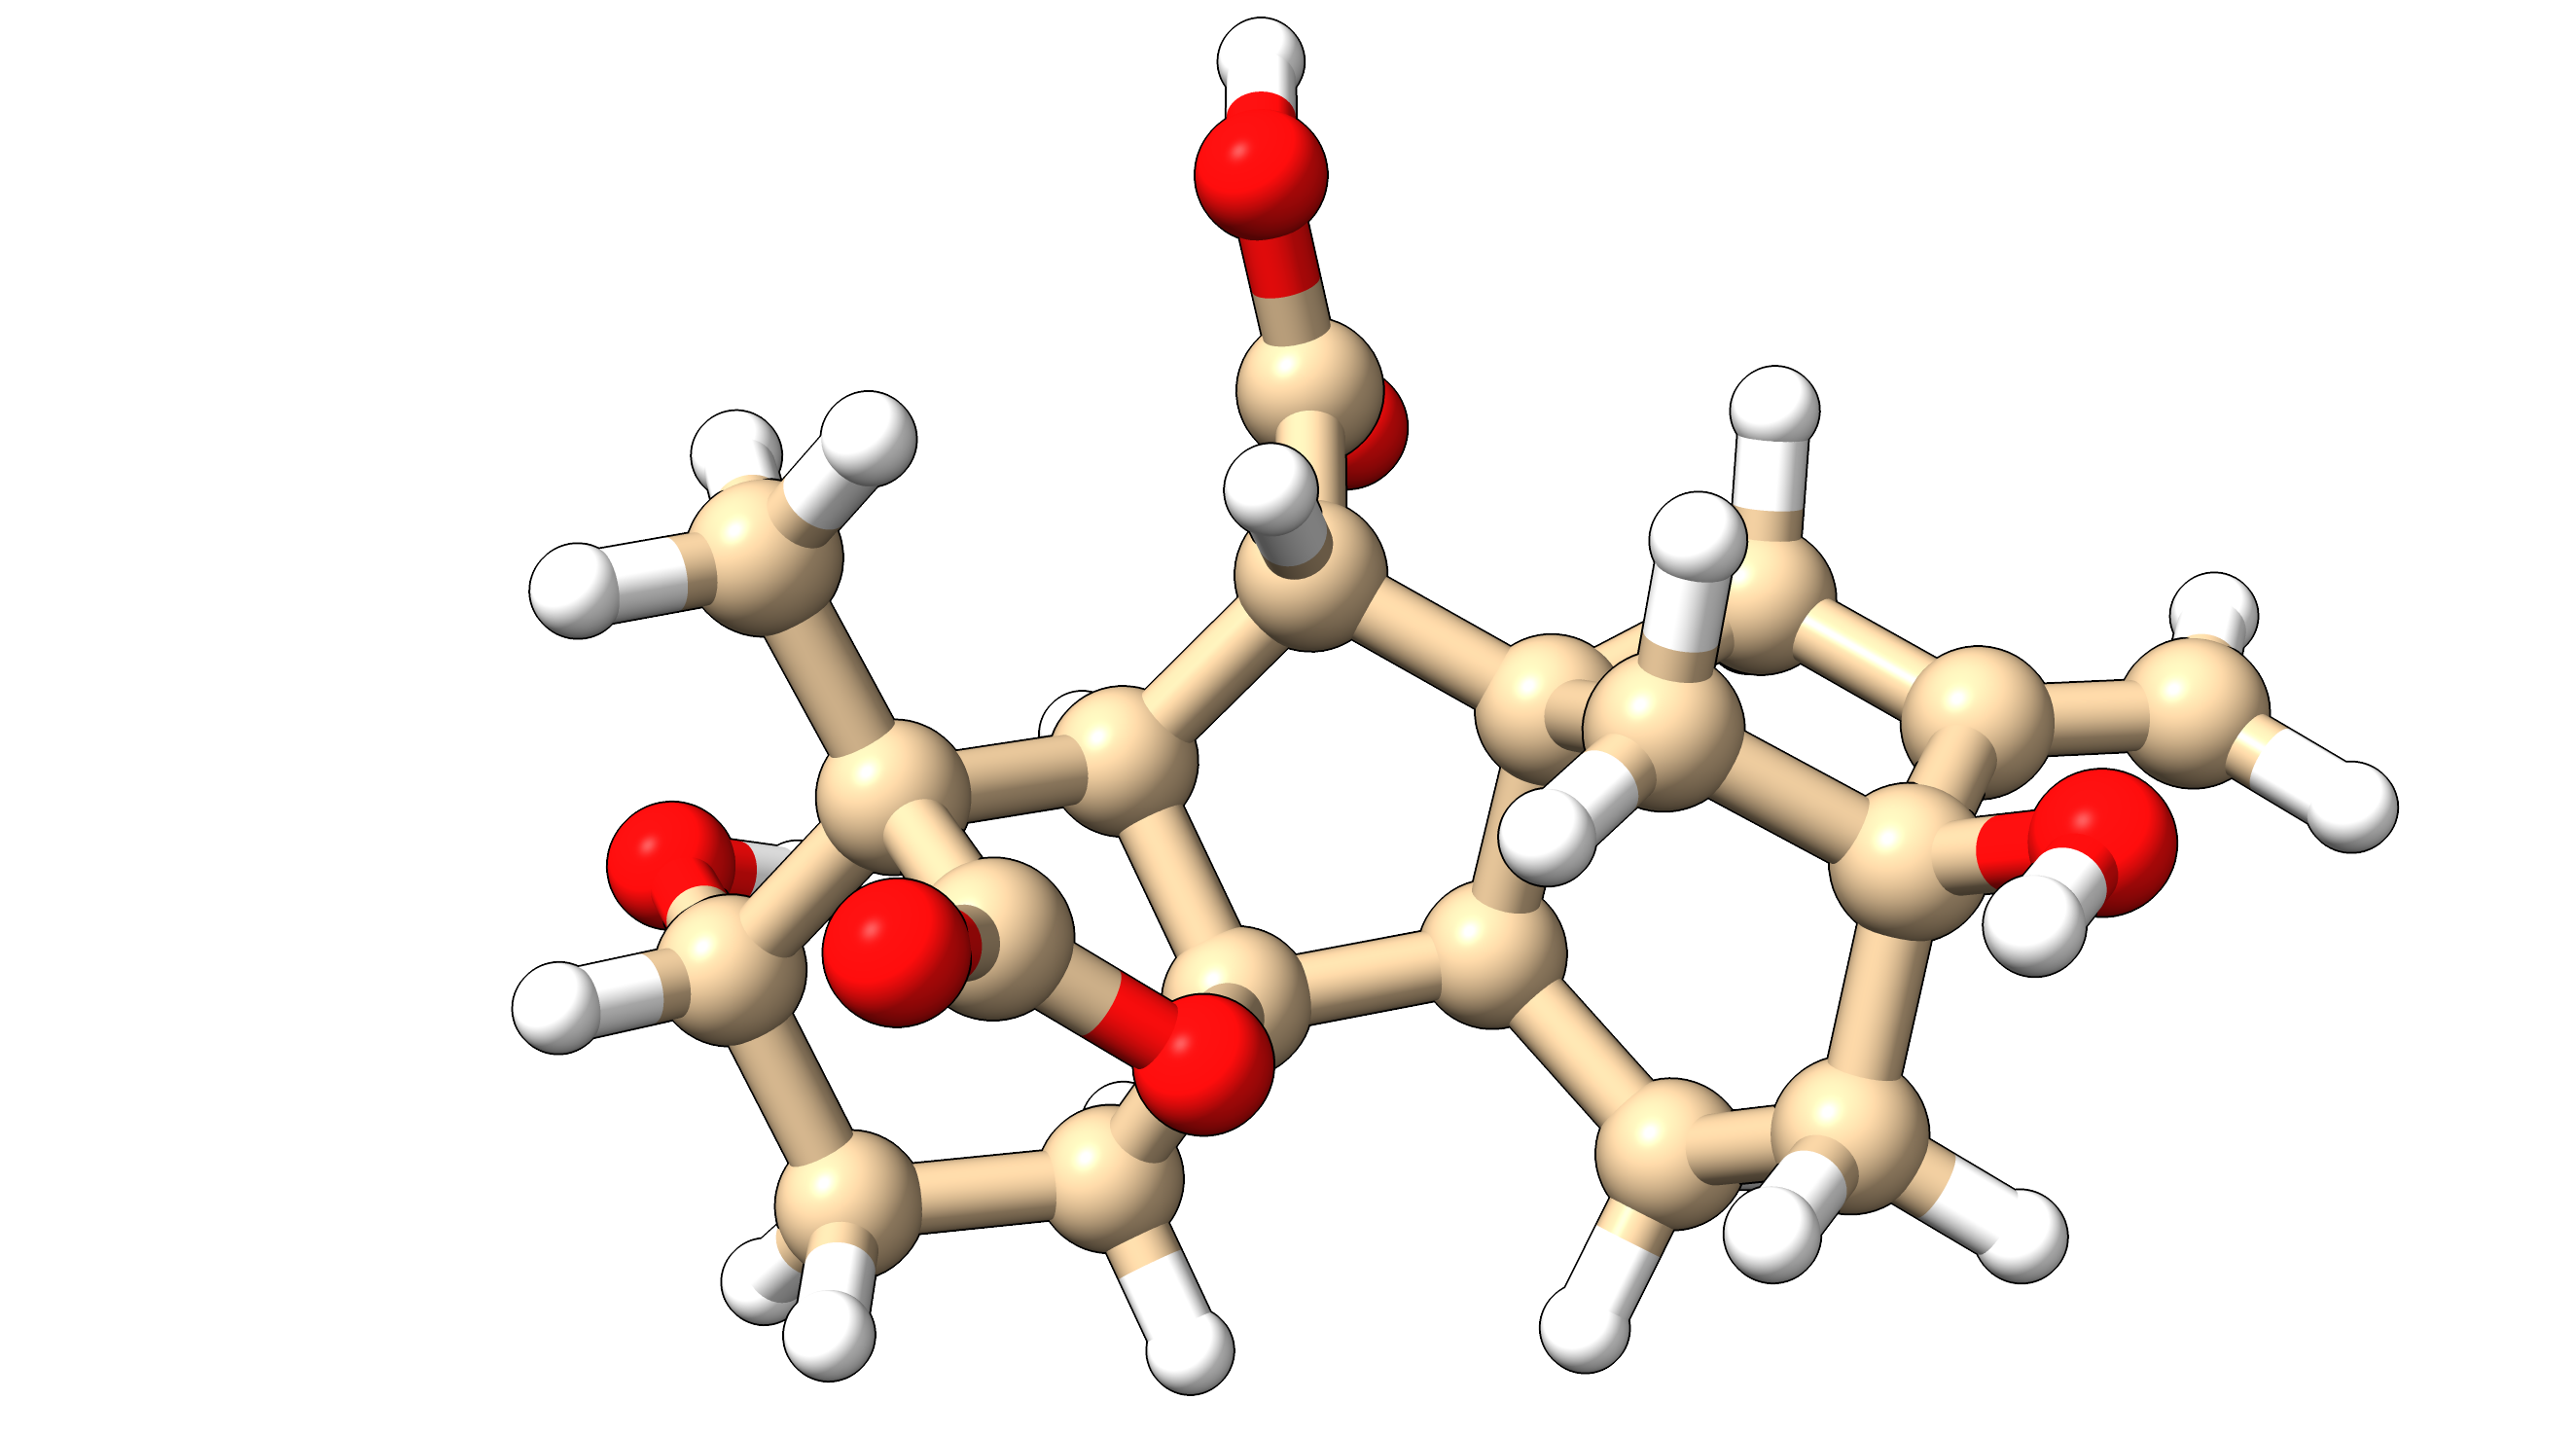
\includegraphics[width=\textwidth]{Gibberellin-A1.png}\\[0.3em]
      {\footnotesize Gibberellin A1 -- C\textsubscript{19}H\textsubscript{24}O\textsubscript{6},
      348.4~g/mol (PubChem CID 5280379)}
    \end{column}
  \end{columns}
\end{frame}

\begin{frame}{Gibberellins -- growth effect}
  \begin{columns}[c]
    \begin{column}{0.55\textwidth}
      \begin{itemize}
        \item GA-deficiency mutants (key oxidase disrupted):
          \begin{itemize}
            \item Smaller but more resilient
            \item \textbf{Higher grain yield}
          \end{itemize}
        \item[$\Rightarrow$] GA-deficiency-linked yield gains underpinned
          the \textbf{Green Revolution} (1970s)
      \end{itemize}
    \end{column}
    \begin{column}{0.42\textwidth}
      \centering
      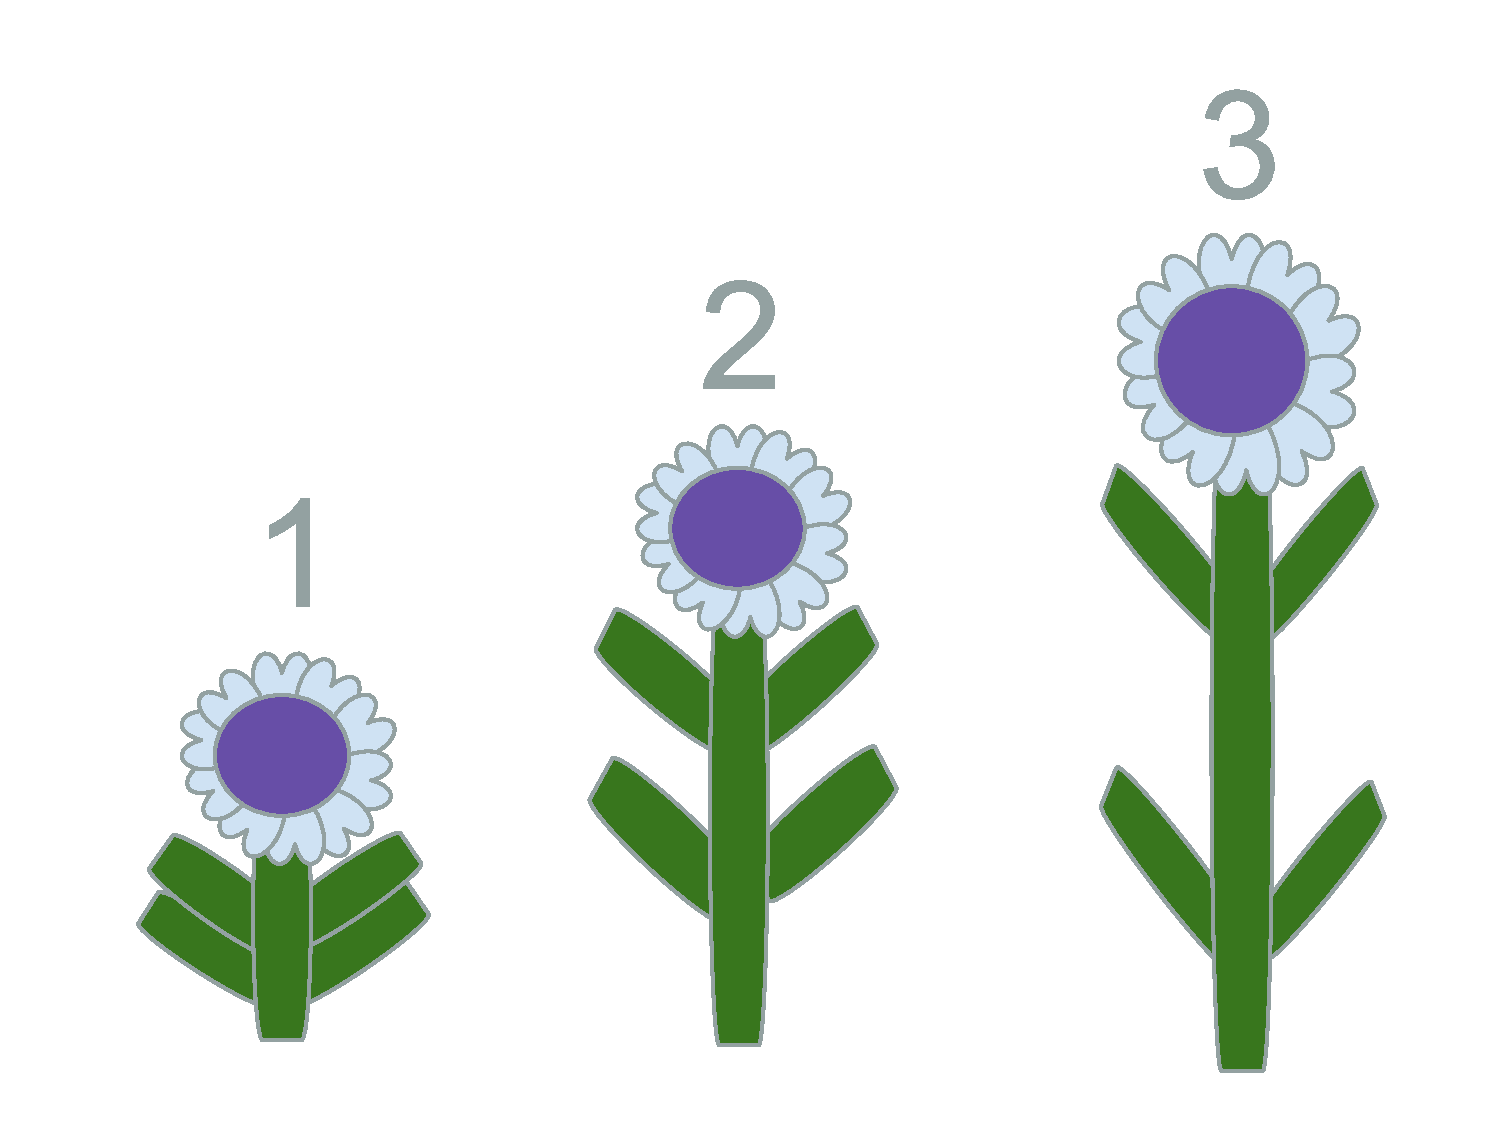
\includegraphics[width=0.75\textwidth]{gibberellin-effect.pdf}\\[0.2em]
      {\scriptsize (1) No gibberellins: dwarf, no internode elongation.
      (2) Average gibberellins: average internode length.
      (3) High gibberellins: long internode length, more stem cell
      division.\\[0.3em]
      Lee Spahr, \textit{The effect of Gibberellins}, CC BY-SA 3.0,
      via Wikimedia Commons (recolored for contrast)}
    \end{column}
  \end{columns}
\end{frame}

\begin{frame}{Nitrate and Peptide Transporters (NPF)}
  \begin{columns}[c]
    \begin{column}{0.46\textwidth}
      \setlength{\leftmargini}{1.1em}\setlength{\leftmarginii}{1.1em}
      \hspace{-0.6em}%
      \begin{itemize}
        \setlength{\itemsep}{0.4em}\setlength{\topsep}{0.4em}
        \item Part of the \textbf{Major Facilitator Superfamily (MFS)}
          of membrane transporters
        \item Transport:
          \begin{itemize}
            \setlength{\itemsep}{0.4em}\setlength{\topsep}{0.4em}
            \item Nitrate (NO\textsubscript{3}\textsuperscript{-})
            \item Dipeptides
            \item Gibberellins
          \end{itemize}
        \item Specific to tissue and substrate
      \end{itemize}
    \end{column}
    \begin{column}{0.52\textwidth}
      \centering
      \colorbox{white}{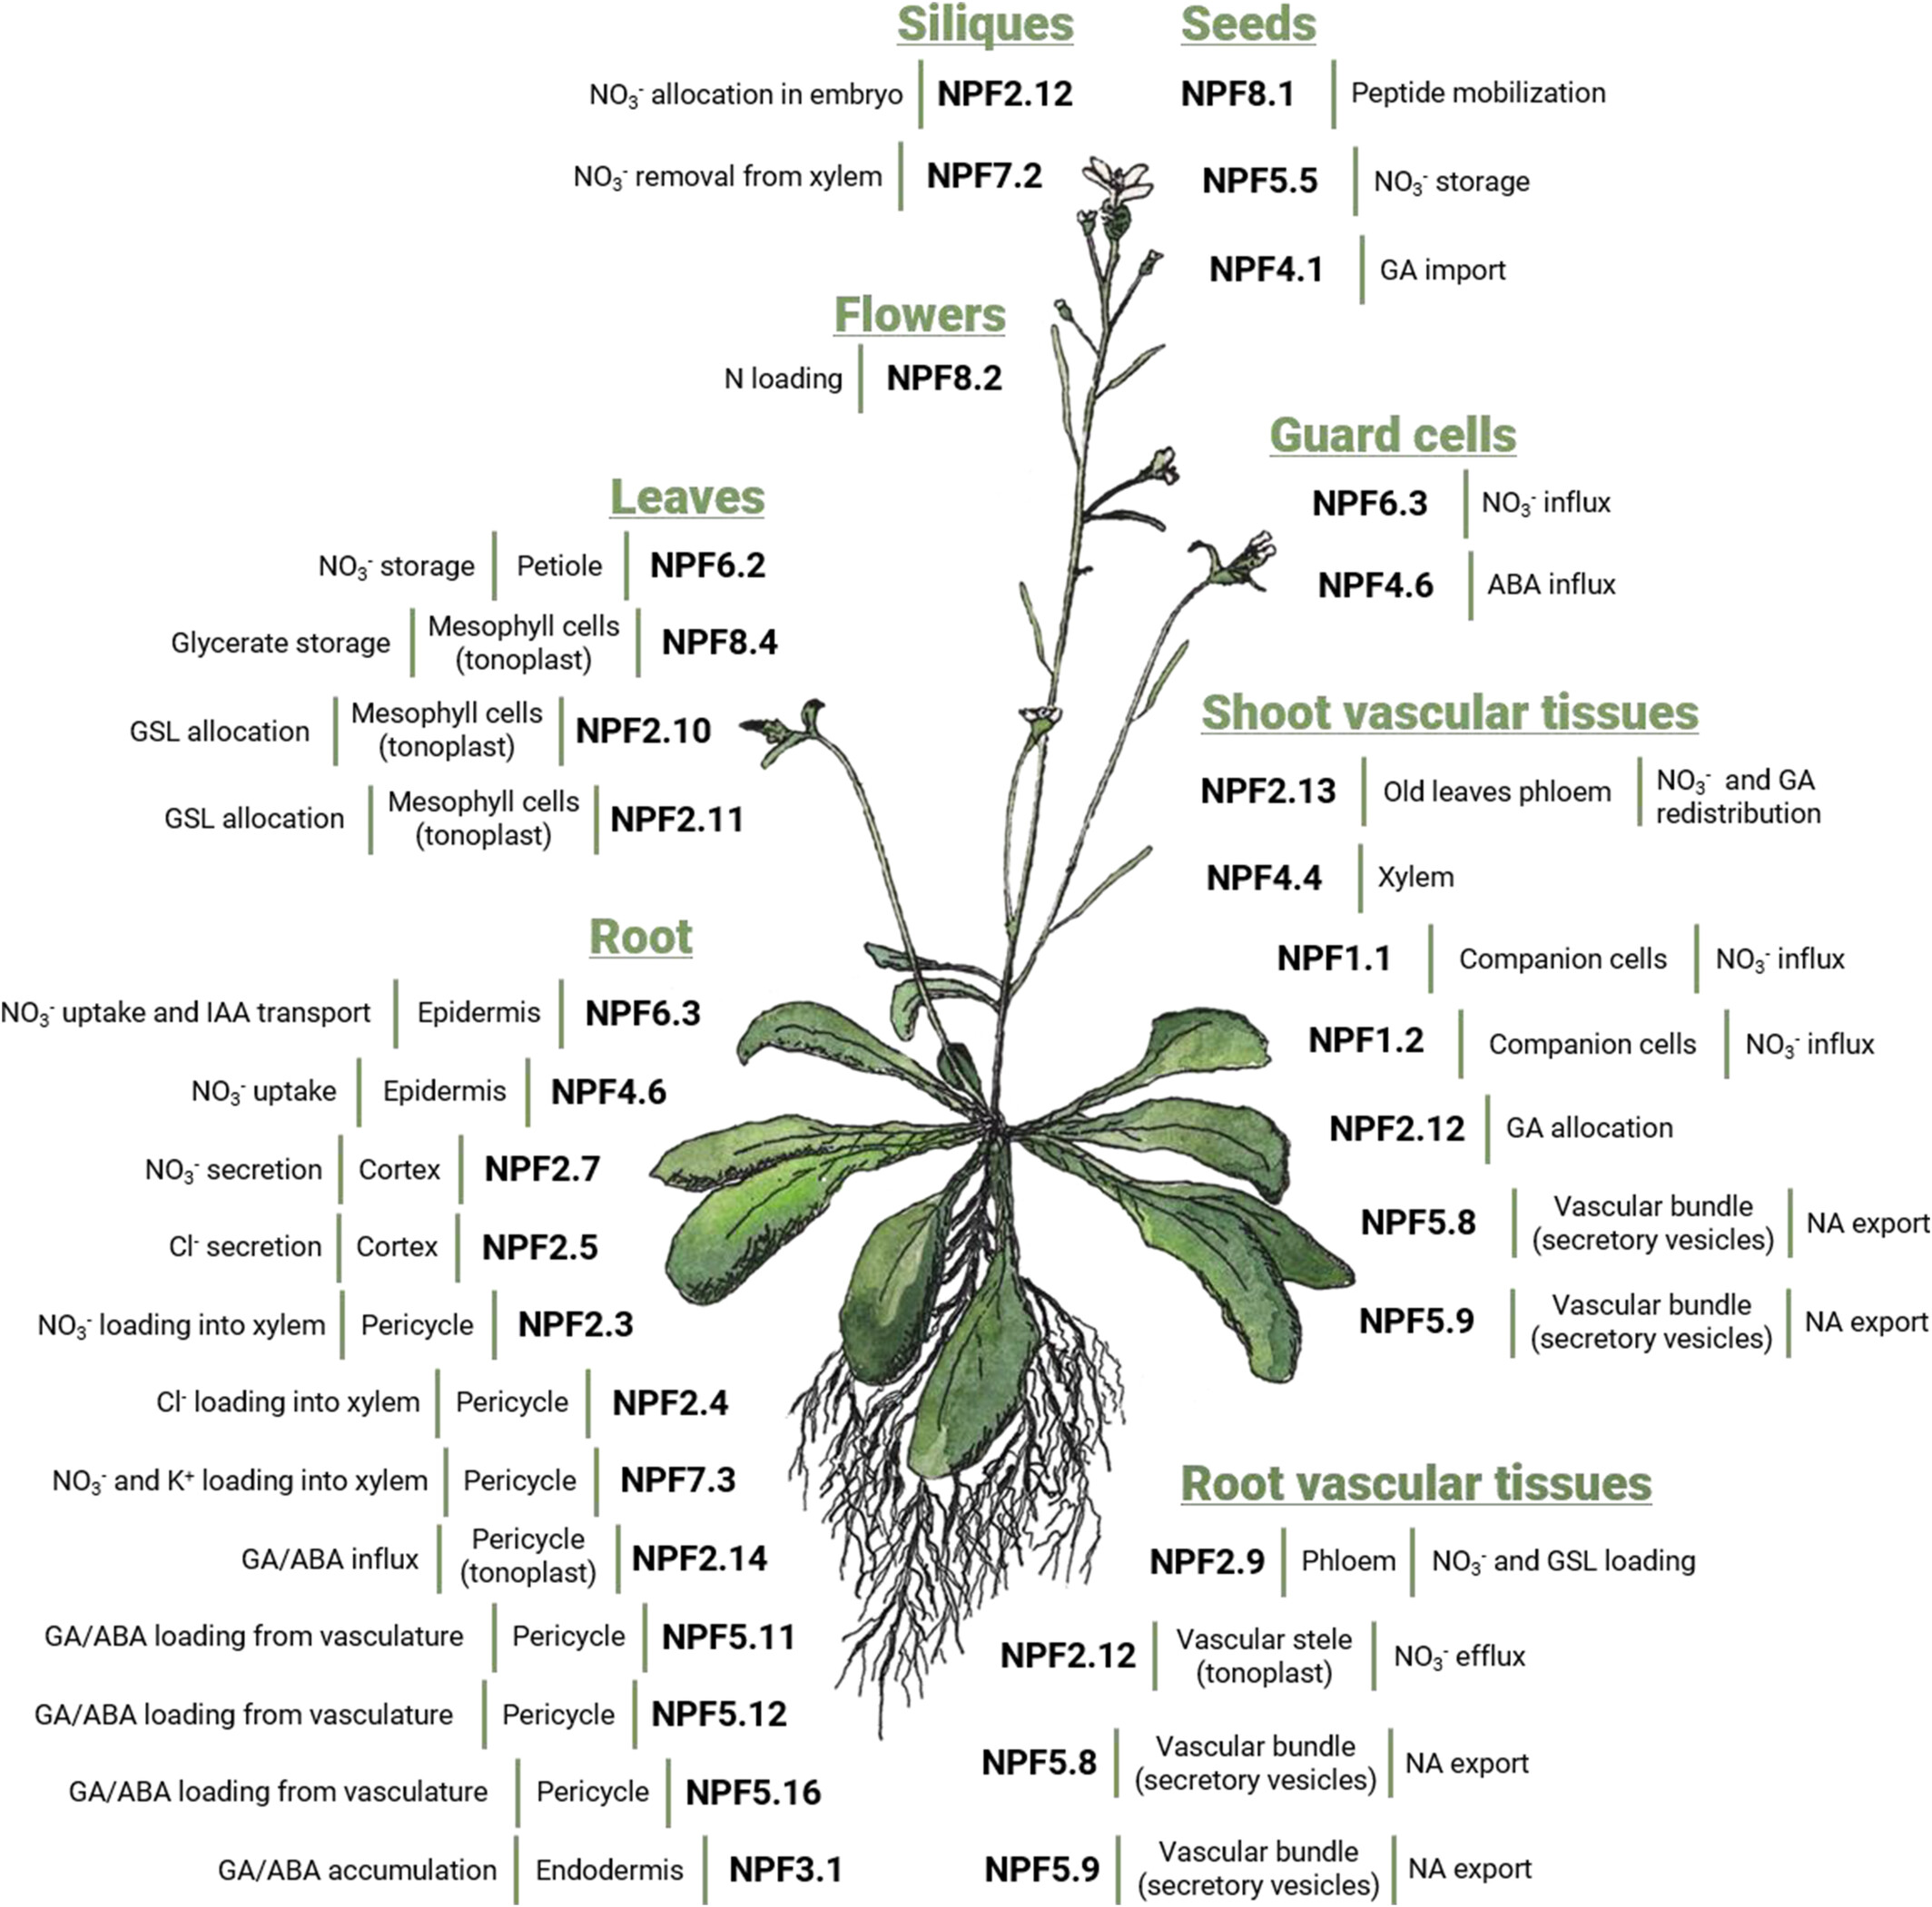
\includegraphics[width=0.76\textwidth]{NPF_tissue_distribution.jpg}}\\[0.1em]
      {\tiny Tissue localization and function of characterized NPFs in
      \textit{Arabidopsis thaliana}; located in the plasma membrane
      unless otherwise indicated. NA, nicotianamine.\\
      Morales de los Ríos \textit{et al.}, \textit{New Phytologist}, CC
      BY 4.0. DOI:10.1111/nph.70730}
    \end{column}
  \end{columns}
\end{frame}

\begin{frame}{MFS transport cycle: six conformations}
  \footnotesize Alternating-access mechanism: transport requires passing
  through a fully \textbf{occluded} intermediate in either direction --
  the \textbf{biological reason} the pipeline targets six conformations
  per protein, not six independent opinions on one.

  \begin{center}
  \resizebox{0.60\textwidth}{!}{%
  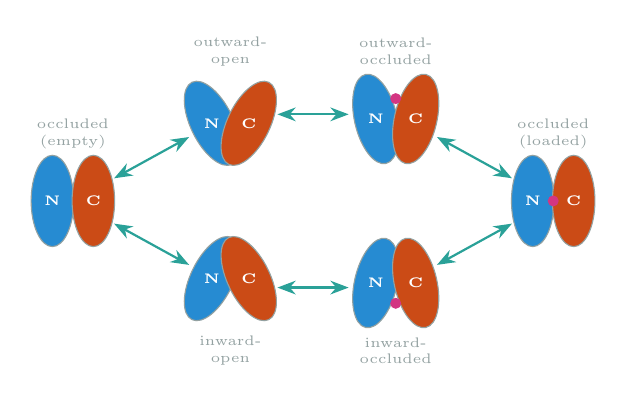
\begin{tikzpicture}[>=Stealth]
    \tikzset{arr/.style={<->, thick, draw=accent}}

    \mfsicon{0}{0}{0}{}
    \mfsicon{2.0}{1.1}{26}{}
    \mfsicon{4.1}{1.1}{13}{\fill[substrate] (0,0.2) circle (0.07);}
    \mfsicon{6.1}{0}{0}{\fill[substrate] (0,0) circle (0.07);}
    \mfsicon{4.1}{-1.1}{-13}{\fill[substrate] (0,-0.2) circle (0.07);}
    \mfsicon{2.0}{-1.1}{-26}{}

    \draw[arr, shorten >=17pt, shorten <=17pt] (0,0) -- (2.0,1.1);
    \draw[arr, shorten >=17pt, shorten <=17pt] (2.0,1.1) -- (4.1,1.1);
    \draw[arr, shorten >=17pt, shorten <=17pt] (4.1,1.1) -- (6.1,0);
    \draw[arr, shorten >=17pt, shorten <=17pt] (6.1,0) -- (4.1,-1.1);
    \draw[arr, shorten >=17pt, shorten <=17pt] (4.1,-1.1) -- (2.0,-1.1);
    \draw[arr, shorten >=17pt, shorten <=17pt] (2.0,-1.1) -- (0,0);

    \node[fgtext, font=\tiny, align=center] at (0,0.85) {occluded\\(empty)};
    \node[fgtext, font=\tiny, align=center] at (2.0,1.9) {outward-\\open};
    \node[fgtext, font=\tiny, align=center] at (4.1,1.9) {outward-\\occluded};
    \node[fgtext, font=\tiny, align=center] at (6.1,0.85) {occluded\\(loaded)};
    \node[fgtext, font=\tiny, align=center] at (4.1,-1.9) {inward-\\occluded};
    \node[fgtext, font=\tiny, align=center] at (2.0,-1.9) {inward-\\open};
  \end{tikzpicture}%
  }
  \end{center}

  {\tiny\color{muted} Redrawn after Drew \textit{et al.}, \textit{Chem.\
  Rev.} 2021, 121, 5289--5335 (Fig.\ 8a), CC BY-NC-ND 4.0 --
  DOI:10.1021/acs.chemrev.0c00983}
\end{frame}

\begin{frame}{What's experimentally known}
  \begin{columns}[c]
    \begin{column}{0.55\textwidth}
      \begin{itemize}
        \item Only \textbf{2 NPFs} have experimentally resolved
          structures:
          \begin{itemize}
            \item NPF6.3 (4OH3, 5A2N, 5A2O)
            \item NPF2.10 (9UI1, 9UI6, 9UIF, 9UIT)
          \end{itemize}
        \item Only \textbf{importers} are well characterized in the
          literature (technical constraints)
        \item \textbf{Exporters} remain unidentified
      \end{itemize}
    \end{column}
    \begin{column}{0.4\textwidth}
      \centering
      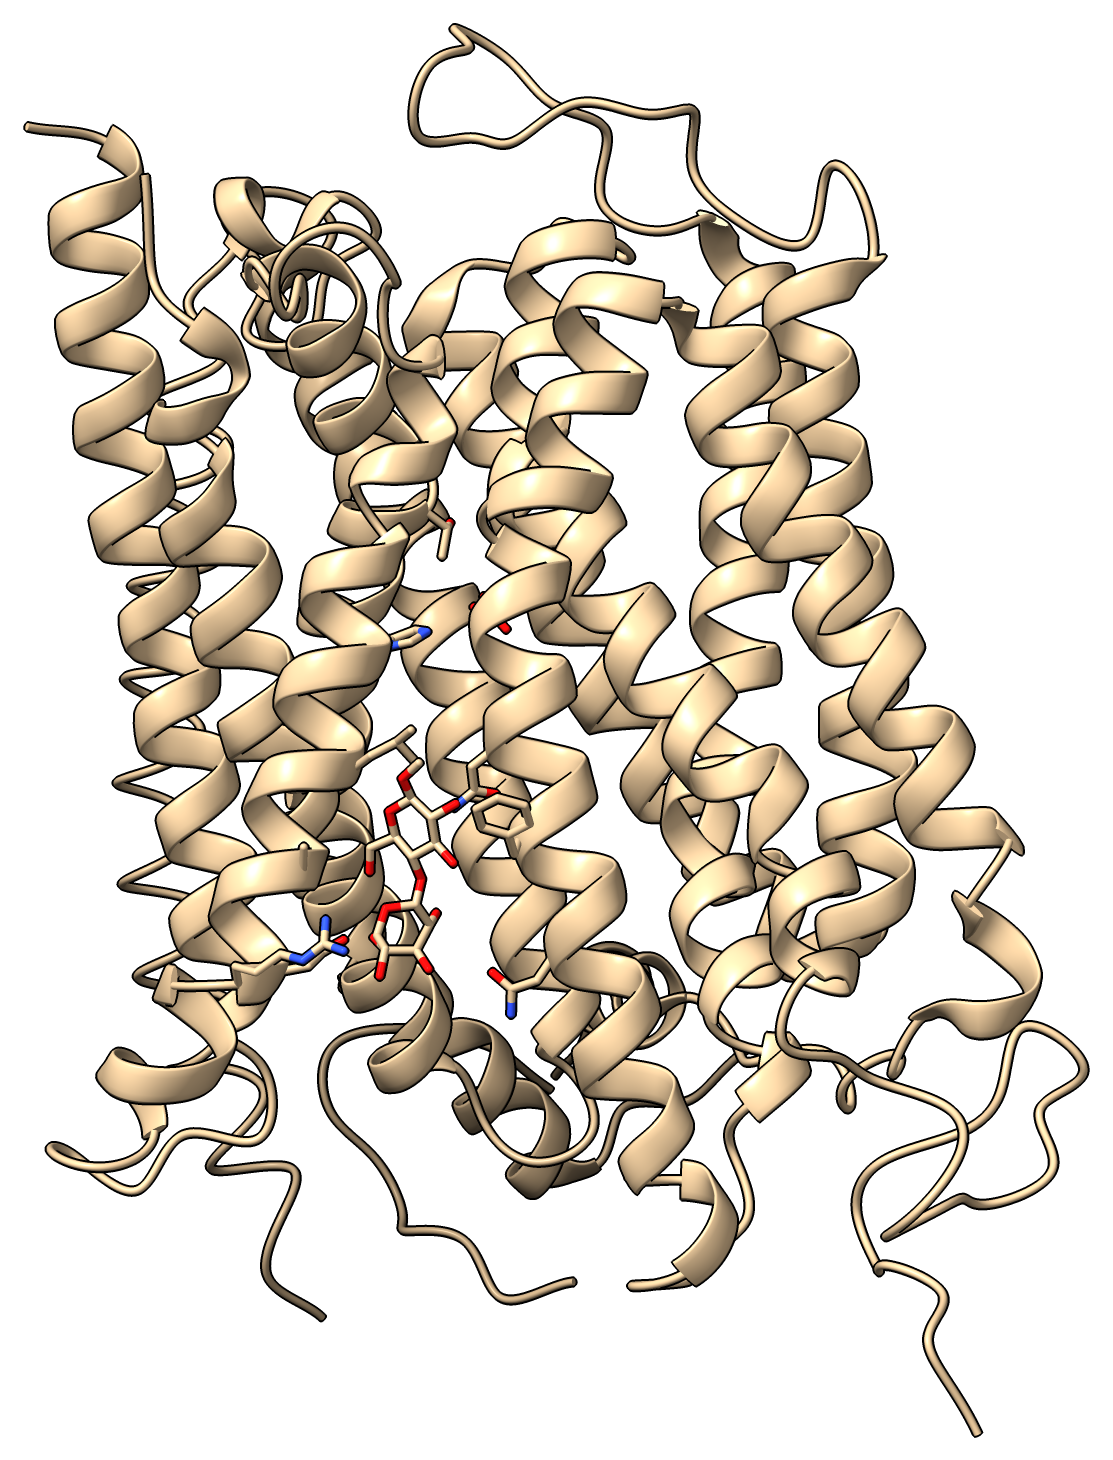
\includegraphics[width=0.8\textwidth]{4OH3-crop.png}\\[0.3em]
      {\footnotesize NPF6.3 -- PDB 4OH3, X-ray, 3.25~\AA\\
      Sun \textit{et al.}, \textit{Nature} 2014}
    \end{column}
  \end{columns}
\end{frame}

\begin{frame}{Research project goals}
  \begin{enumerate}
    \item \textbf{Ab initio modelling of 3D structures}
      \begin{enumerate}
        \item Pipeline to generate the six conformations \hfill
          {\small\textit{(this project)}}
        \item Network interaction analysis (ligand and intra-chain)
      \end{enumerate}
    \item \textbf{Functional annotation of NPFs}
      \begin{enumerate}
        \item Identify key features of importers vs.\ non-importers
        \item Eventually, find exporters
      \end{enumerate}
  \end{enumerate}
\end{frame}

% ---------------------------------------------------------------------
\section{Motivation}
% ---------------------------------------------------------------------

\begin{frame}{The question}
  \begin{itemize}
    \item Arabidopsis \textbf{NPF} (Nitrate/Peptide Transporter) family
      \item[] % TODO: one line on the biological question driving this
        \textit{Which conformations can each NPF transporter adopt, apo and
        ligand-bound?}
    \item Structure prediction as a proxy for conformational sampling
  \end{itemize}
\end{frame}

\begin{frame}{Why not just one model?}
  \begin{itemize}
    \item Sibling repo \texttt{AF3\_NPF\_pipeline} already sampled
      \textbf{30 AF3 seeds/protein}
    \item Overlaying those ensembles with Boltz-2 (Gibberellin importers,
      8 proteins) showed: AF3 alone \textbf{does not} recover every
      conformation a second, architecturally-different model finds
    \item[$\Rightarrow$] One model isn't enough -- run \textbf{six together}
      instead of resampling one
  \end{itemize}
\end{frame}

\begin{frame}{The six backends}
  \begin{columns}[T]
    \begin{column}{0.5\textwidth}
      \begin{itemize}
        \item AlphaFold3
        \item Boltz-2
        \item Chai-1
      \end{itemize}
    \end{column}
    \begin{column}{0.5\textwidth}
      \begin{itemize}
        \item OpenFold3
        \item Protenix
        \item RosettaFold3
      \end{itemize}
    \end{column}
  \end{columns}
  \vspace{1em}
  \centering
  All launched \textbf{together} per protein via ABCfold's
  \texttt{abcfold -abcopr} against the \emph{same} resolved fold input.
\end{frame}

% ---------------------------------------------------------------------
\section{Pipeline overview}
% ---------------------------------------------------------------------

\begin{frame}{Three stages}
  \centering
  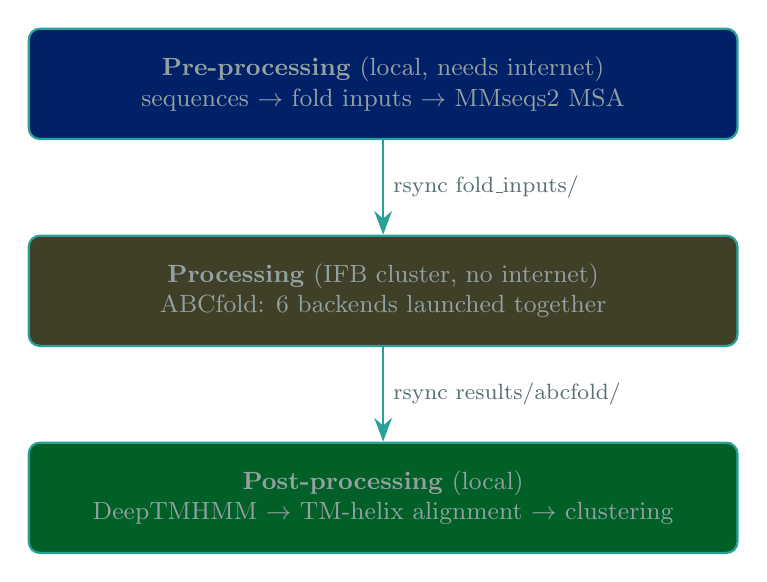
\begin{tikzpicture}[
      every node/.style={text=fgtext},
      stage/.style={draw=accent, thick, rounded corners, minimum width=9cm, minimum height=1.4cm,
                     align=center, font=\small},
      arr/.style={-{Stealth[length=3mm]}, thick, draw=accent}
    ]
    \node[stage, fill=blue!25!bgdark] (pre)  {\textbf{Pre-processing} (local, needs internet)\\
                                        sequences $\to$ fold inputs $\to$ MMseqs2 MSA};
    \node[stage, fill=orange!25!bgdark, below=1.2cm of pre] (proc) {\textbf{Processing} (IFB cluster, no internet)\\
                                        ABCfold: 6 backends launched together};
    \node[stage, fill=green!25!bgdark, below=1.2cm of proc] (post) {\textbf{Post-processing} (local)\\
                                        DeepTMHMM $\to$ TM-helix alignment $\to$ clustering};
    \draw[arr] (pre) -- (proc) node[midway, right, text=muted] {\footnotesize rsync fold\_inputs/};
    \draw[arr] (proc) -- (post) node[midway, right, text=muted] {\footnotesize rsync results/abcfold/};
  \end{tikzpicture}
\end{frame}

% ---------------------------------------------------------------------
\section{Pre-processing}
% ---------------------------------------------------------------------

\begin{frame}{Stage 1--3: from sequence to resolved fold input}
  \begin{enumerate}
    \item \textbf{Sequences} -- UniProt $\to$ per-protein FASTA
    \item \textbf{Fold input} -- \texttt{fold\_input.json} per protein
      $\times$ apo/holo (AF3-dialect JSON, ABCfold's native input:
      sequence + every replica seed)
    \item \textbf{MMseqs2 default run} -- MSA + top-hit templates from the
      ColabFold webserver, no manual curation, no pocket restraint;
      embedded into \texttt{fold\_input.resolved.json}
  \end{enumerate}
  \vspace{0.5em}
  \small Runs locally, driven by Snakemake
  (\texttt{worflows/preprocessing/Snakefile}); resumable -- existing
  resolved inputs are never re-fetched.
\end{frame}

% ---------------------------------------------------------------------
\section{Processing}
% ---------------------------------------------------------------------

\begin{frame}{Stage 4: ABCfold on the IFB cluster}
  \begin{itemize}
    \item One \texttt{abcfold -abcopr\ldots} call per protein $\times$ form
    \item Launches all 6 backends against the same
      \texttt{fold\_input.resolved.json}
    \item AlphaFold3 backend runs via IFB's \texttt{alphafold} module
      (Singularity wrapper, auto-discovered) -- no separate image needed
    \item Boltz/Chai-1/OpenFold3/Protenix/RosettaFold3 built once via
      \texttt{--prime} on a login node (needs internet)
  \end{itemize}
\end{frame}

\begin{frame}{Gibberellin importers run first}
  \begin{itemize}
    \item 8 GA1-ligand proteins (\texttt{NPF2.1, NPF2.5, NPF2.10, NPF2.12,
      NPF2.13, NPF3.1, NPF4.1, NPF5.6}) -- the group already studied with
      AF3 + Boltz-2
    \item Listed in \texttt{priority\_gibberellin.txt}, put first in the
      SLURM array manifest
    \item Fastest path to validating the six-backend approach against a
      known result
  \end{itemize}
\end{frame}

% ---------------------------------------------------------------------
\section{Post-processing}
% ---------------------------------------------------------------------

\begin{frame}{Stage 5--6: topology and alignment}
  \begin{enumerate}
    \item \textbf{DeepTMHMM} -- TM-helix topology (BioLib), once
    \item \textbf{TM-helix Kabsch alignment} -- per protein $\times$ form,
      pooled across every backend and seed
  \end{enumerate}
  \vspace{0.5em}
  Output: \texttt{results/tm\_alignment/<protein>/\{aligned\_ca\_tm.npy,
  meta.csv\}} -- \texttt{meta.csv} now carries a \textbf{\texttt{model}}
  column (\texttt{alphafold3}/\texttt{boltz}/\texttt{chai1}/
  \texttt{openfold3}/\texttt{protenix}/\texttt{rosettafold3}).
\end{frame}

\begin{frame}{Stage 7: clustering \& visualisation}
  \begin{itemize}
    \item Notebook-based (JupyterLab, \texttt{envs/notebook.yaml})
    \item Same schema as \texttt{AF3\_NPF\_pipeline}'s clustering notebooks
      + one new axis: \textbf{color/facet by backend}
    \item \emph{That's the whole point of this pipeline}: which backend(s)
      actually reach which conformational cluster?
    \item Status: % TODO -- not yet ported / in progress / done?
  \end{itemize}
\end{frame}

% ---------------------------------------------------------------------
\section{Status \& next steps}
% ---------------------------------------------------------------------

\begin{frame}{Where we are}
  \begin{itemize}
    \item % TODO: which stages have run on real data so far
    \item % TODO: any results worth showing (a cluster plot?)
    \item % TODO: known issues worth flagging (e.g. SMILES escaping fix in af3\_to\_boltz.py, backend backfill caveat)
  \end{itemize}
\end{frame}

\begin{frame}{Next steps}
  \begin{itemize}
    \item % TODO
    \item % TODO
  \end{itemize}
\end{frame}

\begin{frame}
  \centering
  \Huge Questions?
\end{frame}

\end{document}
